\documentclass[letterpaper]{article} % 
\usepackage{pgfplots} % 画折线图
\usepackage{scalefnt} %用于设置字体

\begin{document}
	
	\begin{figure}[h] %插入图片
		\centering %图片居中
		\resizebox{0.8\columnwidth}{!}{  %用于修改图片大小
			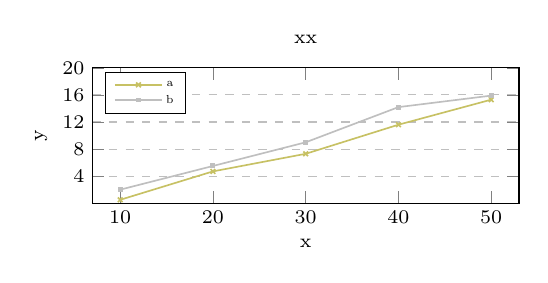
\begin{tikzpicture} %tikz图片
			\scalefont{0.7} %设置字体大小
			\begin{axis}[
			sharp plot, %控制线的风格
			title=xx,%图像标题
			xmode=normal,% 控制坐标轴为线性
%			ymode=log,% 控制坐标轴为对数
			xlabel=x, %x坐标名
			ylabel=y, %y坐标名
			width=7cm, height=3.3cm,  %设置长和宽
			xmin=0.7, xmax=5.3,  % 设置x坐标范围
			ymin=0, ymax=20,  % 设置y坐标范围
			xtick={1, 2, 3, 4, 5},  %指定x轴刻度值。如果为空,则自动设置刻度线。即分割坐标轴
			xticklabels={10, 20, 30, 40, 50}, %指定x轴刻度标签
			ytick={4, 8, 12, 16, 20}, %指定y轴刻度值。如果为空,则自动设置刻度线。即分割坐标轴
			xlabel near ticks, % 设置x坐标名位置靠近折线图
			ylabel near ticks, % 设置y坐标名位置靠近折线图
			ymajorgrids=true, % 启用/禁用 [公式] 轴上刻度线位置上的网格线
			grid style=dashed, % 设置网格线格式
			legend pos=north west, % 设置折线对应标签的位置
			legend style={nodes={scale=0.6, transform shape}},  % 设置折线标签的格式
			]
			
			%画第一条线,semithick设置线的粗细为0.6pt,mark是折线标示形状,options是mark形状的大小 , olive!50!white是颜色,coordinates中包含要绘制的点的坐标
			\addplot+[semithick,mark=x,mark options={scale=0.6}, olive!50!white] plot coordinates { 
				(1, 0.5)
				(2, 4.7)
				(3, 7.3)
				(4, 11.6)
				(5, 15.3)
			};
			\addlegendentry{a}%第一条线标签
			
			%画第二条线
			\addplot+[semithick,mark options={scale=0.3}, lightgray] plot coordinates {
				(1, 2.0)
				(2, 5.5)
				(3, 9.0)
				(4, 14.2)
				(5, 15.9)
			};
			\addlegendentry{b} %第二条线标签

			\end{axis}
			\end{tikzpicture}
		}
		\caption{xxxx} % 设置caption
		\label{fig:label}  % 设置用于reference的label
	\end{figure}

\end{document}

